

\section{Introduction}

In the realm of sports betting, football stands out as an ideal focus for developing predictive and optimization models due to its global popularity and the abundance of available data. The rich historical datasets, comprehensive statistics, and extensive coverage make football a fertile ground for data-driven analysis. By concentrating on football, we can leverage vast amounts of information to build robust models that capture the nuances of the game, ultimately enhancing the accuracy of predictions and the effectiveness of betting strategies.

This chapter provides a comprehensive overview of the system architecture designed to implement the theoretical framework outlined earlier. We present the various components of the system, describe how they interact, and explain the workflows involved in data collection, storage, processing, and presentation. The goal is to give the reader a clear understanding of how the theoretical concepts are translated into a practical, working solution before delving into the specifics of the inference and optimization modules in subsequent chapters.

\section{General System Architecture}

The system is designed with modularity and scalability in mind, adhering to a microservices architecture \cite{Newman2015} that allows individual components to operate independently and communicate through well-defined interfaces. This approach facilitates maintenance, testing, and future enhancements.

\subsection{Components Overview}

The system comprises the following primary components:

\begin{itemize}
    \item \textbf{Data Collection Module}: Responsible for gathering historical and real-time data on football matches and betting odds from various sources.
    \item \textbf{Database}: Centralized storage for all collected data, predictions, and optimization results.
    \item \textbf{Prediction Module}: Utilizes machine learning models to estimate the probabilities of different match outcomes.
    \item \textbf{Optimization Module}: Computes optimal betting strategies based on the selected utility function and model predictions.
    \item \textbf{Model Monitoring Module}: Monitors training of inference models.
    \item \textbf{User Interface (UI) and Backend}: Provides users with access to data, predictions, and betting recommendations through a web-based platform.
    \item \textbf{Scheduler}: Automates the execution of tasks such as data collection, model retraining, and optimization at predefined intervals.
    \item \textbf{APIs}: Facilitate communication between components, ensuring seamless data flow and integration.
\end{itemize}

\subsection{Interactions Between Components}

The interactions between the components are orchestrated to ensure efficient data processing and timely updates:

\begin{enumerate}
    \item The \textbf{Data Collection Module} retrieves data from external sources and stores it in the \textbf{Database}.
    \item The \textbf{Prediction Module} trains models and infers probabilities on asked outcomes using data from the  \textbf{Database} and storing the results in the  \textbf{Database}. The training of the models is monitored using the \textbf{Model Monitoring Module} which stores the models metrics into the \textbf{Database}.
    \item The \textbf{Optimization Module} calculates optimal betting fractions based on the predictions and current odds stored in the \textbf{Database} using a given strategy.
    \item The \textbf{User Interface} fetches data from the \textbf{Database} via the \textbf{Backend} and presents it to the user.
    \item The \textbf{Scheduler} triggers data collections, training, inference and optimisation using the APIs from \textbf{Data Collection Module}, \textbf{Prediction} and \textbf{Optimization Module} at specified times scheduled.
\end{enumerate}

\begin{figure}[H]
    \centering
    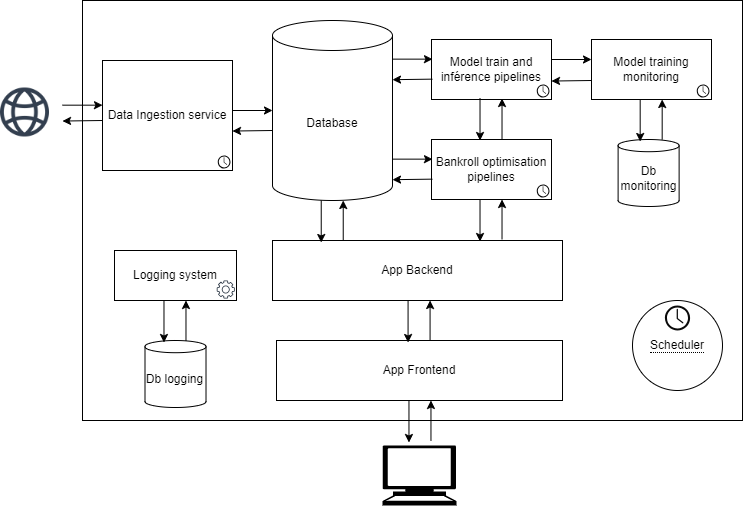
\includegraphics[width=0.8\textwidth, keepaspectratio]{images/Architecture_optimsportbet.png}
    \caption{Architecture of the system}
    \label{fig:elo_score_5_teams_during_time}
\end{figure}


\section{Data Collection}

Accurate and comprehensive data collection is vital for building reliable predictive models and effective betting strategies. The goal is to build an historical database which continues to build with real time relevant data.

\subsection{Data Sources Used}

We utilize a variety of reputable sources to gather data:

\begin{itemize}
    \item \textbf{Football Match Data}: Historical match results, match schedule, team statistics, player performance metrics, and other relevant information are sourced using scrapping on two websites: 
    \begin{itemize}
        \item \hyperlink{https://fbref.com/en/}{FBref}: For historical match results and coming match schedule.
        \item \hyperlink{https://sofifa.com/}{SoFifa}: For teams and players past and current ratings and statistics.
    \end{itemize}
    \item \textbf{Odds Data}: Betting odds are collected from multiple bookmakers through one API.
    \begin{itemize}
        \item \hyperlink{https://the-odds-api.com/}{The Odds API}: The free tier credits allows to perform 500 requests per month on various sports, bookmakers and leagues to retrieve the current odds. Historical odds data are not included.
    \end{itemize}
\end{itemize}


\subsection{Collection Methods}

Data is collected using a combination of methods:

\paragraph{Web Scraping}

A fork of the \hyperlink{https://soccerdata.readthedocs.io/en/latest/}{Soccerdata} python library, has been adapted to scrape data from websites that do not provide APIs (FBref, SoFifa). 

\paragraph{APIs}

For sources that offer APIs (The Odds API), we integrate with them using HTTP requests to fetch structured data efficiently.

\paragraph{Data Pre-processing}

Collected data undergoes a very simple pre-processing to ensure consistency and usability:

\begin{itemize}
    \item \textbf{Data type conversion}: Adapting the type of the data to the most adapted type.
    \item \textbf{Unity}: Only inserting new data in the database, or filling None values of existing data (for instance, the score of a match is only available after the match is played 
    \item \textbf{Integration}: Aligning data from different sources for seamless storage and analysis.
\end{itemize}

\section{Data Storage}

A robust data storage solution is essential for managing the diverse datasets involved.

\subsection{Database Choice}

We opted for a relational database management system (RDBMS), specifically \textit{PostgreSQL}, due to its reliability, scalability, and support for complex queries.

\subsection{Data Model}

The database schema is designed to reflect the relationships between different types of data:

\subsubsection{Tables}

\begin{itemize}
    \item `\textbf{fbref\_results}`: Each row corresponds to a match (historic and coming), with league, date and time of the match, both team and score if match is finished and the result is available and fetched from FBref website.
    \item `\textbf{sofifa\_teams\_stats}`: Each row corresponds to a a team and a date of update with metrics and categorical values that represent at best the team at the moment of the update (overall score, attack, build\_up\_speed ...).
    \item `\textbf{soccer\_odds}`: Each row corresponds to a match, a bookmaker, an outcome with its odd at a given update time. There is also information about the commence time of the match, the league, the home and away team names, the type of odd...
    \item `\textbf{models\_results}`: Each row corresponds to a match, the inference results of the model, the date-time of inference and the model used, with additional information such as the date and tile of the match and home and away team.
    \item `\textbf{optim\_results}`: Each row corresponds to a game, a date time of optimisation, the model used for inference, the best odds for each outcome found across a pool of bookmaker as well as the bookmakers names of each odds chose and the fraction of the bankroll to invest given utility function. There is additional information such as the probability inferred and used by the optimiser, the date-time of inference of these probabilities, the date and time of the match...
\end{itemize}


\begin{figure}[H]
    \centering
    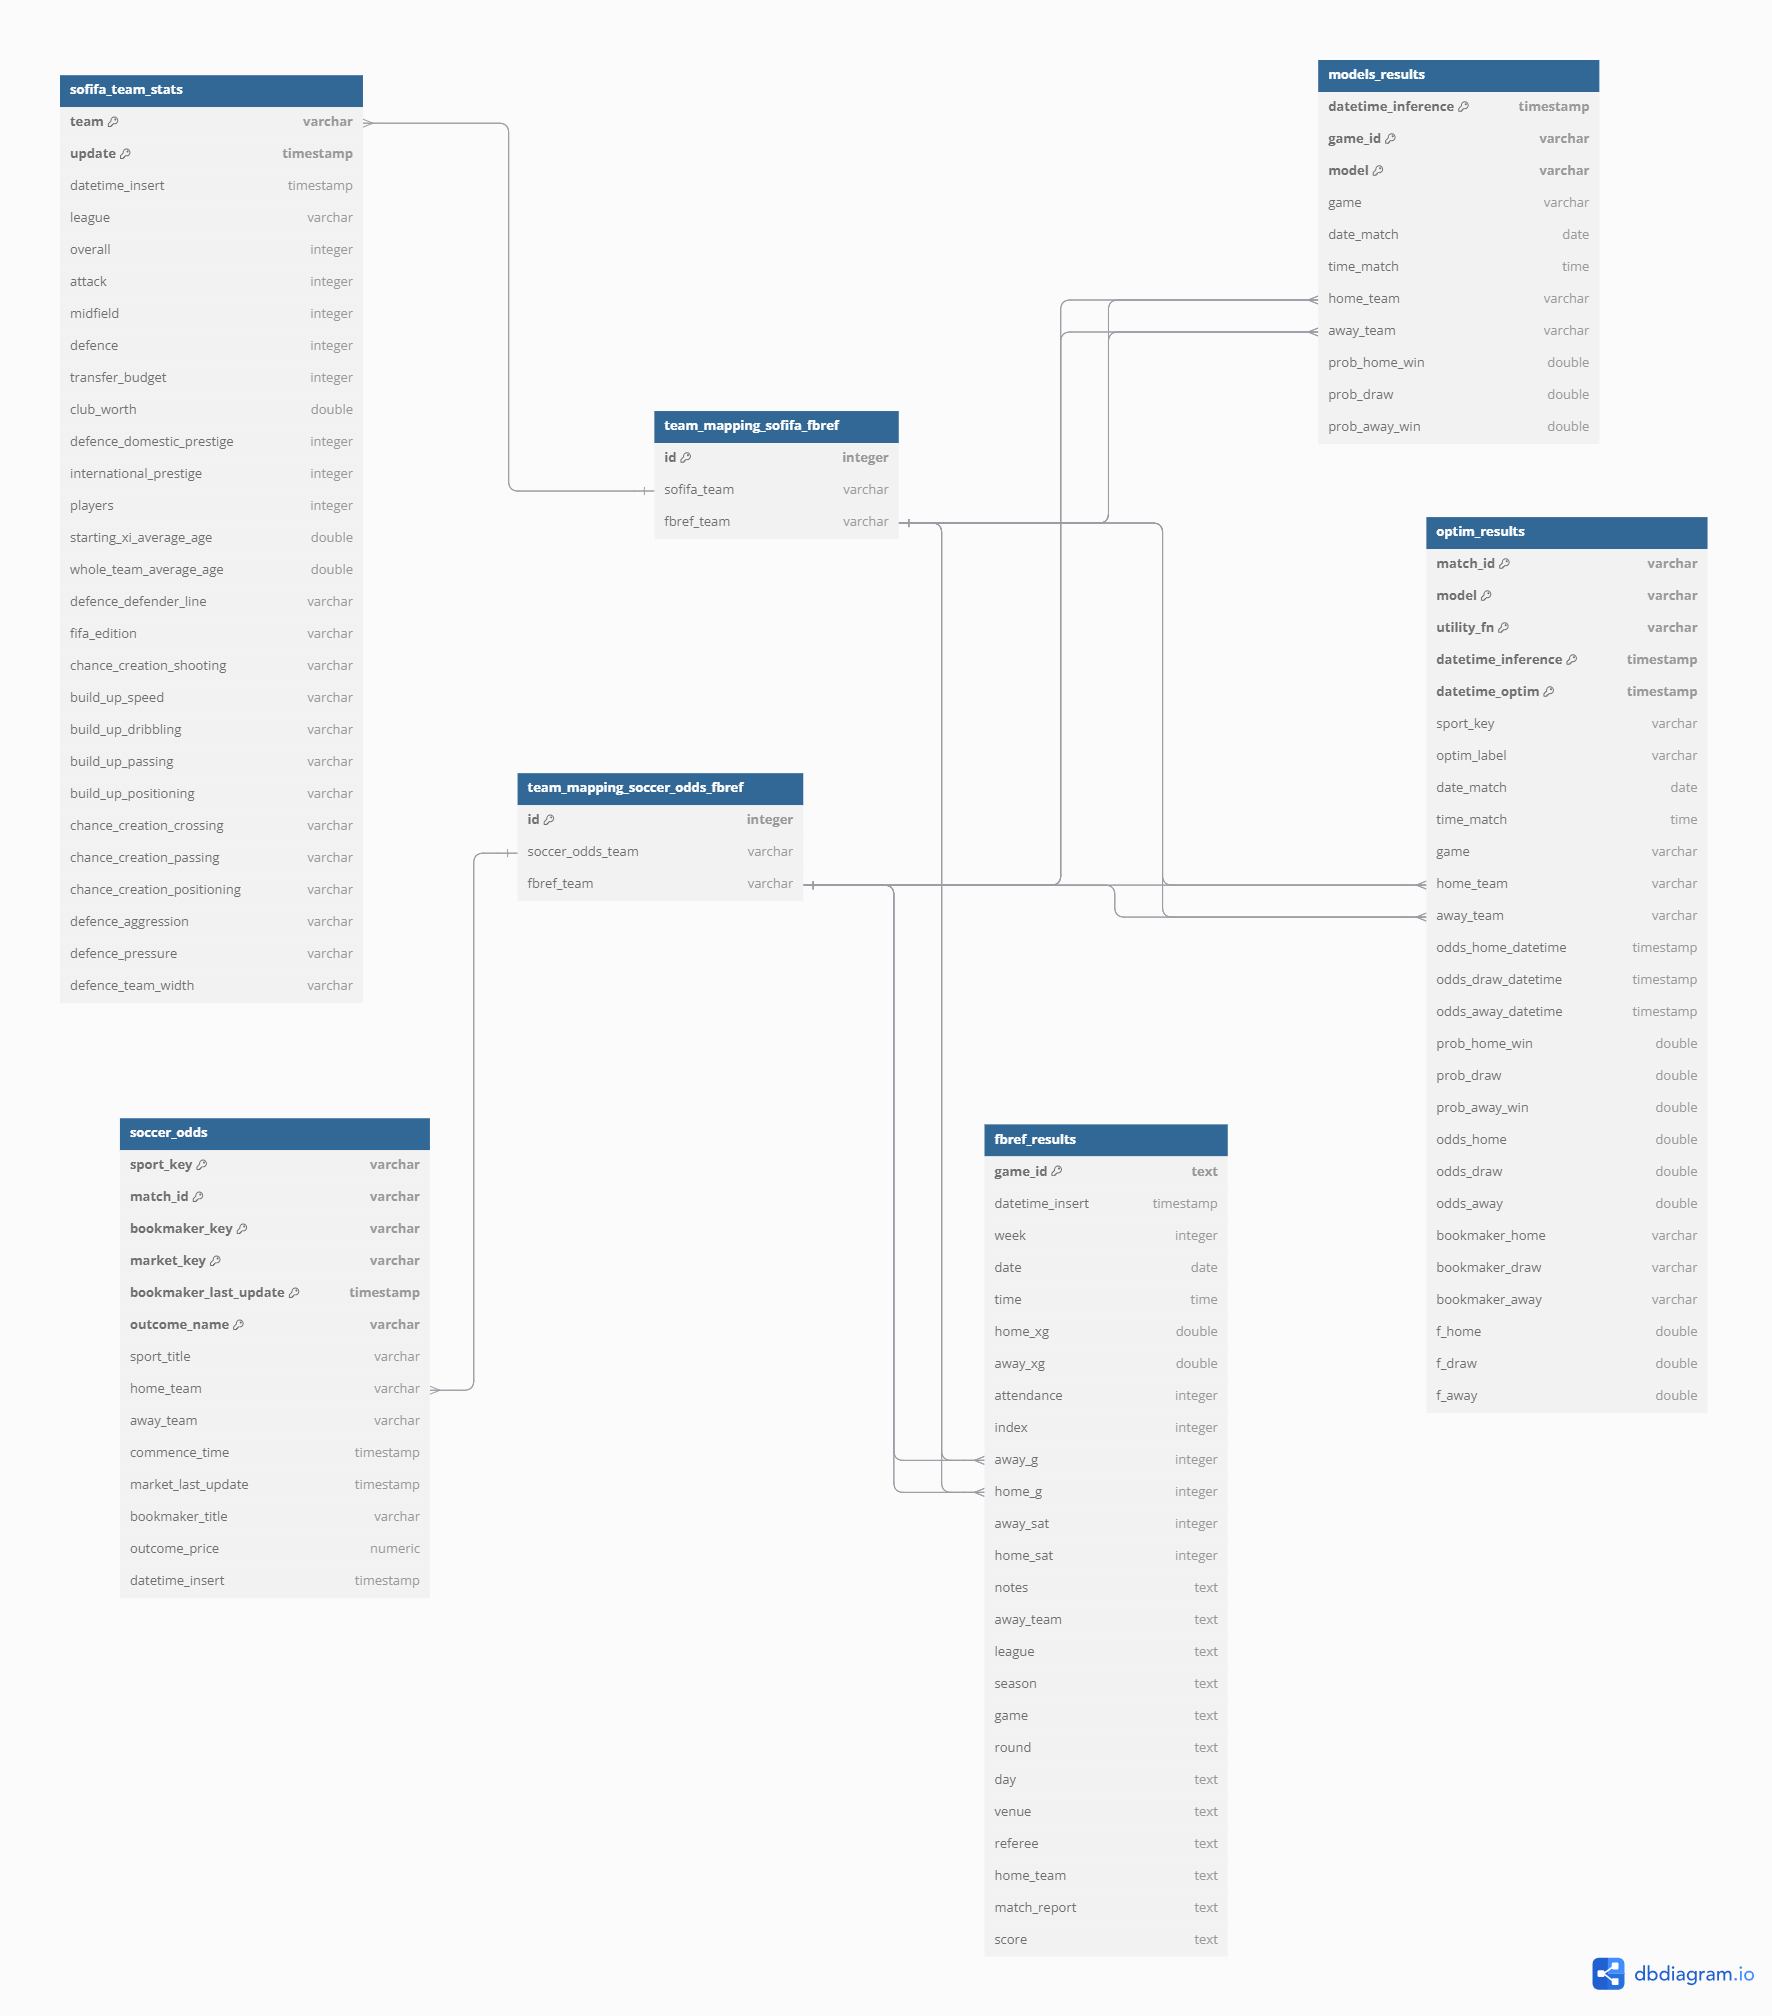
\includegraphics[width=0.8\textwidth, keepaspectratio]{images/db_uml.png}
    \caption{UML diagram of the database}
    \label{fig:uml_db}
\end{figure}

\section{Module Overview}

The system incorporates several modules, each performing specific functions within the overall architecture.

\subsection{Data Collection Module}

As described earlier, this module is responsible for fetching and pre-processing data from various sources.

\subsection{Prediction Module}

Although detailed discussion is deferred to a later chapter, this module uses machine learning algorithms to predict the probabilities of different match outcomes based on historical data.

\subsection{Optimization Module}

This module calculates optimal betting strategies by applying mathematical optimization techniques to the predictions and odds data. The specifics of the optimization algorithms and utility functions will be explored in a subsequent chapter.

\subsection{Scheduler}

The scheduler automates the execution of tasks such as data collection, model retraining, inference, and optimization. It ensures that the system remains up-to-date with the latest data and predictions.

\subsection{User Interface and Backend}

The user interface provides a platform for users to access data, view predictions, and interact with the system. The backend handles user requests, processes data, and communicates with other modules via APIs.

\section{User Interface and Monitoring}

\subsection{User Interface Design}

The UI is designed to be intuitive and user-friendly, providing clear visualizations and easy navigation.

\paragraph{Features}

\begin{itemize}
    \item \textbf{Dashboard}: Displays key metrics, including upcoming matches, predicted probabilities, and recommended betting strategies.
    \item \textbf{Historical Data Access}: Allows users to explore past matches, predictions, and outcomes.
    \item \textbf{Customization}: Users can select preferred bookmakers according to their interests.
\end{itemize}

\subsection{Monitoring}

System health and performance are monitored continuously:

\begin{itemize}
    \item \textbf{Logging}: Activity logs are maintained for debugging and audit purposes.
    \item \textbf{Alerts}: Notifications are sent in case of errors or significant events.
\end{itemize}


\section{Conclusion}

This chapter provided an overview of the system architecture implemented to realize the theoretical framework developed earlier. By focusing on football, we leverage abundant data to build predictive models and optimize betting strategies. The modular design, utilizing microservices and APIs,ensures scalability and flexibility. The database serves as the central repository, integrating data from various sources and supporting the different modules. The user interface offers a gateway for users to access the system's functionalities. In the subsequent chapters, we will delve into the specifics of the prediction and optimization modules, as well as the deployment strategy using Kubernetes and containerization technologies.
